\newpage
\section{Appendix}
\subsection{Appendix A}
In this appendix we present the visualisation of some clusters obtained by the K-means and GMM algorithms. Results can be found in Figures \ref{fig:embeddingsKMeans} and \ref{fig:embeddingsGMM} respectively. Similarly to Figure 3 from the original paper, we conclude that our clusters have clear semantic meaning, both for K-means and GMMs. 

\begin{figure}[h]
\centering
    \subfloat[Indian women with dark hair]{\includegraphics[width=0.45\linewidth]{images_and_figures/kmeans_indian_females.pdf}}
    \subfloat[Male African sportsmen]{\includegraphics[width=0.45\linewidth]{images_and_figures/kmeans_african_males_sporty.pdf}}
 \\
    \subfloat[Young Asian women with red hair and bangs]{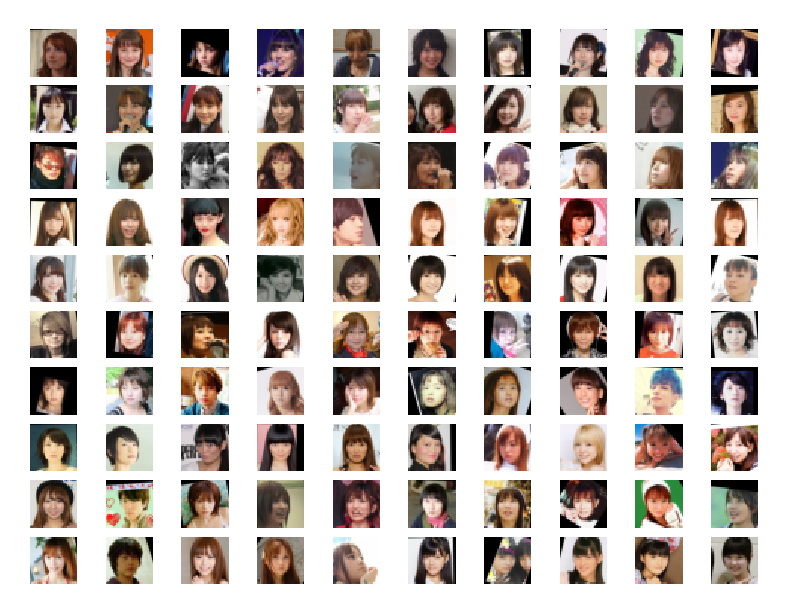
\includegraphics[width=0.45\linewidth]{images_and_figures/kmeans_asian_females_redhair.pdf}}	
    \subfloat[Caucasian men with short dark hair]{\includegraphics[width=0.45\linewidth]{images_and_figures/kmeans_caucasian_males_shorthair.pdf}}
    \caption{Examples of clusters obtained with the K-means algorithm (\textit{K}=100) on the RFW dataset based on the feature embeddings computed with the FaceNet (Webface) model, labelled with potential semantic classes (labelled by us).}
  \label{fig:embeddingsKMeans}
\end{figure}

\begin{figure}[h]
\centering
    \subfloat[Older Asian men]{\includegraphics[width=0.45\linewidth]{images_and_figures/gmm_asian_men_older.pdf}}
    \subfloat[Blonde Caucasian women]{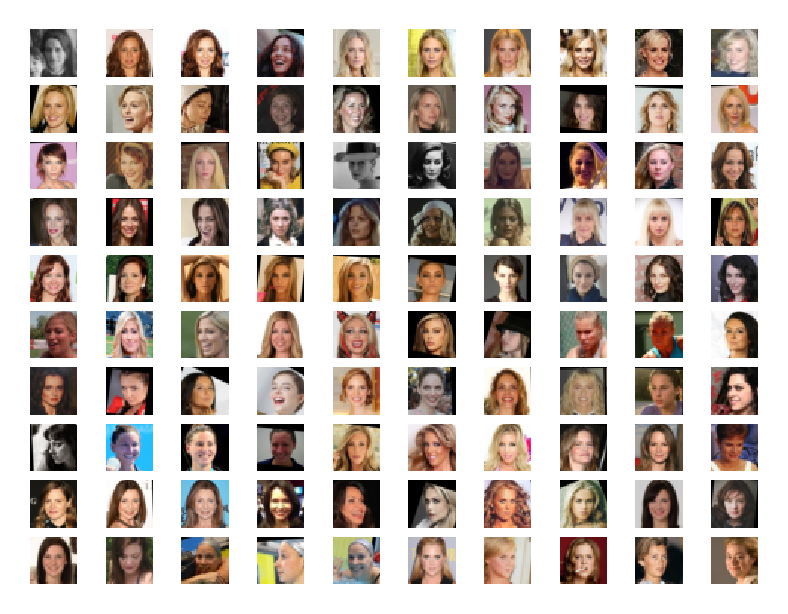
\includegraphics[width=0.45\linewidth]{images_and_figures/gmm_caucasian_blonde_females.pdf}}
 \\
    \subfloat[Indian men with mustache]{\includegraphics[width=0.45\linewidth]{images_and_figures/gmm_indian_men_mustache.pdf}}	
    \subfloat[Young Indian women]{\includegraphics[width=0.45\linewidth]{images_and_figures/gmm_indian_women_young.pdf}}
    \caption{Examples of clusters obtained with the GMM algorithm (k = 100) on the RFW dataset based on the feature embeddings computed with the FaceNet (VGGFace2) model, labelled with potential semantic classes (labelled by us).}
  \label{fig:embeddingsGMM}
\end{figure}

\newpage 
 
\subsection{Appendix B}
We present additional figures of the experiments on the other methods used by the original authors: the Adverserial Gender De-biasing algorithm (AGENDA) \citep{DBLP:journals/corr/abs-2006-07845}, the Fair Score Normalization (FSN) method \citep{TERHORST2020332}, and Oracle (introduced by the original authors). For clarity, we also include the results for Baseline, FairCal with K-means and FairCal with GMM. Results can be found in Tables \ref{tab:AccAp}, \ref{tab:FairCalAp} and \ref{tab:appPredEq}.

\begin{table}
\footnotesize
\centering
\begin{tabular}{l l ll ll ll}
\toprule
&& \multicolumn{2}{c}{AUROC} & \multicolumn{2}{c}{TPR @ 0.1\% FPR} & \multicolumn{2}{c}{TPR @ 1\% FPR} \\
RFW & &  Authors  &   Ours   & Authors &  Ours   & Authors & Ours \\
\midrule
\multirow{5}{5em}{FaceNet (VGGFace2)} 
& AGENDA      &  76.83$\pm$0.57 &  79.12$\pm$0.67 &    8.32$\pm$1.86 &  13.33$\pm$2.87 &   18.01$\pm$1.44 &  21.63$\pm$2.56 \\
& Baseline    &  88.26$\pm$0.19 &  89.97$\pm$0.58 &   18.42$\pm$1.28 &  25.27$\pm$6.51 &   34.88$\pm$3.27 &  39.92$\pm$2.40 \\
& FairCal     &  90.58$\pm$0.29 &  92.17$\pm$0.40 &   23.55$\pm$1.82 &  26.93$\pm$5.23 &   41.88$\pm$1.99 &  49.68$\pm$2.40 \\
& FSN         &  90.05$\pm$0.29 &  91.30$\pm$0.35 &   23.01$\pm$2.00 &  26.79$\pm$4.63 &   40.21$\pm$2.09 &  44.52$\pm$2.91 \\
& Oracle      &  89.74$\pm$0.31 &  91.26$\pm$0.50 &   21.40$\pm$3.54 &  25.45$\pm$6.20 &  411.83$\pm$2.98 &  47.98$\pm$4.92 \\
& FairCal-GMM &           -- &  92.46$\pm$0.43 &            -- &  29.88$\pm$4.34 &           -- &  50.86$\pm$3.42 \\
\hline
\multirow{5}{5em}{FaceNet (Webface)} 
& AGENDA      &  74.51$\pm$0.94 &  72.79$\pm$1.36 &    6.38$\pm$0.78 &   6.89$\pm$3.27 &  14.98$\pm$1.11 &  13.97$\pm$2.58 \\
& Baseline    &  83.95$\pm$0.22 &  84.46$\pm$0.47 &   11.18$\pm$3.45 &  11.14$\pm$5.34 &  26.04$\pm$2.11 &  26.45$\pm$4.90 \\
& FairCal     &  86.71$\pm$0.25 &  86.97$\pm$0.72 &   20.64$\pm$3.09 &  19.23$\pm$3.64 &  33.13$\pm$1.67 &  33.82$\pm$4.55 \\
& FSN         &  85.84$\pm$0.34 &  86.24$\pm$0.63 &   17.33$\pm$3.01 &  17.98$\pm$5.74 &  32.90$\pm$1.03 &  31.68$\pm$2.02 \\
& Oracle      &  85.23$\pm$0.18 &  85.72$\pm$0.54 &   16.71$\pm$1.98 &  16.72$\pm$2.82 &  31.60$\pm$1.08 &  32.20$\pm$4.37 \\
& FairCal-GMM &           -- &  87.19$\pm$0.53 &            -- &  20.49$\pm$5.36 &           -- &  33.44$\pm$4.09 \\
\\\midrule\\
BFW \\
\midrule
\multirow{5}{5em}{FaceNet (Webface)} 
& AGENDA      &  82.42$\pm$0.45 &  76.33$\pm$0.76 &   15.95$\pm$1.53 &   6.84$\pm$0.72 &  32.51$\pm$1.24 &  18.58$\pm$1.25 \\
& Baseline    &  96.06$\pm$0.16 &  94.62$\pm$0.17 &   33.61$\pm$2.10 &  27.93$\pm$2.02 &  58.87$\pm$0.92 &  52.79$\pm$1.74 \\
& FairCal     &  96.90$\pm$0.17 &  95.67$\pm$0.13 &   46.74$\pm$1.49 &  37.68$\pm$0.87 &  69.21$\pm$1.19 &  60.21$\pm$1.09 \\
& FSN         &  96.77$\pm$0.20 &  94.84$\pm$0.22 &   47.11$\pm$1.23 &  37.87$\pm$0.98 &  69.92$\pm$1.01 &  59.86$\pm$1.23 \\
& Oracle      &  97.28$\pm$0.13 &  96.18$\pm$0.10 &   45.13$\pm$1.45 &  35.34$\pm$1.02 &  67.56$\pm$1.05 &  58.99$\pm$1.01 \\
& FairCal-GMM &           -- &  95.48$\pm$0.15 &            -- &  35.39$\pm$1.46 &           -- &  58.49$\pm$1.57 \\
\hline
\multirow{5}{5em}{ArcFace} 
& AGENDA      &  95.09$\pm$0.55 &  93.17$\pm$0.54 &   69.61$\pm$2.40 &  44.97$\pm$3.06 &  79.67$\pm$2.06 &  64.09$\pm$2.38 \\
& Baseline    &  97.41$\pm$0.34 &  97.34$\pm$0.36 &   86.27$\pm$1.09 &  84.75$\pm$1.26 &  90.11$\pm$0.87 &  89.51$\pm$0.98 \\
& FairCal     &  97.44$\pm$0.34 &  97.37$\pm$0.35 &   86.28$\pm$1.24 &  84.95$\pm$1.32 &  90.14$\pm$0.86 &  89.55$\pm$1.01 \\
& FSN         &  97.35$\pm$0.33 &  97.32$\pm$0.35 &   86.19$\pm$1.13 &  84.77$\pm$1.20 &  90.06$\pm$0.84 &  89.49$\pm$0.98 \\
& Oracle      &  98.91$\pm$0.12 &  98.85$\pm$0.13 &   86.41$\pm$1.19 &  84.98$\pm$1.24 &  90.40$\pm$0.91 &  89.87$\pm$1.06 \\
& FairCal-GMM &           -- &  97.35$\pm$0.37 &            -- &  84.78$\pm$1.21 &           -- &  89.51$\pm$1.00 \\
\bottomrule
\end{tabular}
\caption{Global \textcolor{Emerald}{\textbf{accuracy}} measured by AUROC, TPR at 0.1\% FPR threshold and TPR at 1\% FPR threshold. Higher is better. Entries indicate mean $\pm$ 1 standard deviation over 5-fold validation.}
\label{tab:AccAp}
\end{table}

\begin{table}
\footnotesize
\centering
\begin{tabular}{l l ll ll ll ll}
\toprule
&& \multicolumn{2}{c}{Mean} & \multicolumn{2}{c}{AAD} & \multicolumn{2}{c}{MAD} & \multicolumn{2}{c}{STD} \\
RFW & &  Authors & Ours & Authors & Ours & Authors & Ours & Authors & Ours \\
\midrule
\multirow{5}{5em}{FaceNet (VGGFace2)} 
& AGENDA       &    7.71 &  8.87  &    3.11 &  2.66  &    6.09 &  4.96  &    3.86 &  3.64  \\
& Baseline     &    6.37 &  7.28  &    2.89 &  2.37  &    5.73 &  4.57  &    3.77 &  3.30  \\
& FairCal      &    1.37 &  3.30  &    0.28 &  0.51  &    0.50 &  0.96  &    0.34 &  0.71  \\
& FSN          &    1.43 &  3.67  &    0.35 &  0.59  &    0.57 &  1.07  &    0.40 &  0.79  \\
& Oracle       &    1.18 &  3.50  &    0.28 &  0.97  &    0.53 &  1.80  &    0.33 &  1.33  \\
& FairCal - GMM &     -- &  1.77  &     -- &  0.60  &     -- &  0.98  &     -- &  0.78  \\
\hline
\multirow{5}{5em}{FaceNet (Webface)} 
& AGENDA       &    7.71 &  8.87  &    3.11 &  2.66  &    6.09 &  4.96  &    3.86 &  3.64  \\
& Baseline     &    6.37 &  7.28  &    2.89 &  2.37  &    5.73 &  4.57  &    3.77 &  3.30  \\
& FairCal      &    1.37 &  3.30  &    0.28 &  0.51  &    0.50 &  0.96  &    0.34 &  0.71  \\
& FSN          &    1.43 &  3.67  &    0.35 &  0.59  &    0.57 &  1.07  &    0.40 &  0.79  \\
& Oracle       &    1.18 &  3.50  &    0.28 &  0.97  &    0.53 &  1.80  &    0.33 &  1.33  \\
& FairCal - GMM &     -- &  1.75  &     -- &  0.48  &     -- &  0.82  &     -- &  0.62  \\
\midrule
\\
BFW & & &  &  &  &  &  &  &  \\
\midrule
\multirow{5}{5em}{FaceNet (Webface)}
& AGENDA       &   13.21 &  14.06  &    6.37 &  4.94  &   12.91 &  14.94  &    7.55 &  6.40  \\
& Baseline     &    6.77 &   5.80  &    3.63 &  2.88  &    5.96 &   6.86  &    4.03 &  3.49  \\
& FairCal      &    3.09 &   3.38  &    1.34 &  1.12  &    2.48 &   2.43  &    1.55 &  1.38  \\
& FSN          &    2.76 &   3.45  &    1.38 &  1.40  &    2.67 &   4.60  &    1.60 &  1.90  \\
& Oracle       &    2.23 &   2.64  &    1.15 &  1.00  &    2.63 &   2.76  &    1.40 &  1.29  \\
& FairCal - GMM &     -- &  3.43  &     -- &  1.40  &     -- &  3.64  &     -- &  1.80  \\
\hline
\multirow{5}{5em}{ArcFace} 
& AGENDA       &    5.14 &  17.43  &    2.48 &  3.43  &    5.92 &  8.85  &    3.04 &  4.27  \\
& Baseline     &    2.57 &   2.36  &    1.39 &  1.15  &    2.94 &  3.15  &    1.63 &  1.47  \\
& FairCal      &    2.49 &   2.17  &    1.30 &  1.04  &    2.68 &  2.87  &    1.52 &  1.32  \\
& FSN          &    2.65 &   2.91  &    1.45 &  1.29  &    3.23 &  4.26  &    1.71 &  1.72  \\
& Oracle       &    1.41 &   2.54  &    0.59 &  0.86  &    1.30 &  2.16  &    0.69 &  1.08  \\
& FairCal - GMM &     -- &  1.58  &     -- &  0.85  &     -- &  2.71  &     -- &  1.13  \\
\bottomrule
\end{tabular}
\caption{\textcolor{Bittersweet}{\textbf{Fairness Calibration}} measured by KS score across sensitive subgroups. Measured by mean, the average absolute deviation from the mean (AAD), maximumum absolute deviation from the mean(MAD) and standard deviation from the mean (STD). Lower is better in all cases.}
\label{tab:FairCalAp}
\end{table}

\begin{table}
\footnotesize
\centering
\begin{tabular}{l l ll ll ll}
% model | approach | aad (2) | mad (2) | std (2)
\toprule
\textbf{Global FPR: 1\%}\\
&& \multicolumn{2}{c}{AAD} & \multicolumn{2}{c}{MAD} & \multicolumn{2}{c}{STD} \\
RFW && Authors & Ours & Authors & Ours & Authors & Ours \\
\midrule
\multirow{5}{5em}{FaceNet (VGGFace2)} 
& AGENDA      &    0.71 &  0.71  &    1.14 &  1.19  &    0.81 &  0.94  \\
& Baseline    &    0.68 &  0.74  &    1.02 &  0.94  &    0.74 &  0.90  \\
& FairCal     &    0.28 &  0.59  &    0.46 &  0.95  &    0.32 &  0.77  \\
& FSN         &    0.37 &  0.42  &    0.68 &  0.77  &    0.46 &  0.58  \\
& Oracle      &    0.40 &  0.44  &    0.69 &  0.75  &    0.45 &  0.58  \\
& FairCal-GMM &     -- &  0.44  &     -- &  0.74  &     -- &  0.59  \\
\hline
\multirow{5}{5em}{FaceNet (Webface)} 
& AGENDA      &    0.73 &  0.89  &    1.08 &  1.26  &    0.78 &  1.10  \\
& Baseline    &    0.67 &  0.68  &    1.23 &  1.21  &    0.79 &  0.91  \\
& FairCal     &    0.29 &  0.33  &    0.57 &  0.53  &    0.35 &  0.44  \\
& FSN         &    0.35 &  0.33  &    0.61 &  0.58  &    0.40 &  0.45  \\
& Oracle      &    0.41 &  0.41  &    0.74 &  0.68  &    0.48 &  0.53  \\
& FairCal-GMM &     -- &  0.32  &     -- &  0.62  &     -- &  0.47  \\
\midrule
\\
BFW & & & & & & &  \\
\midrule
\multirow{5}{5em}{FaceNet (Webface)} 
& AGENDA      &    1.21 &  0.63  &    3.09 &  1.43  &    1.51 &  0.81  \\
& Baseline    &    2.42 &  1.99  &    7.48 &  6.30  &    3.22 &  2.85  \\
& FairCal     &    0.80 &  0.60  &    1.79 &  1.52  &    0.95 &  0.81  \\
& FSN         &    0.87 &  0.72  &    2.19 &  1.71  &    1.05 &  0.96  \\
& Oracle      &    0.77 &  0.67  &    1.71 &  1.43  &    0.91 &  0.84  \\
& FairCal-GMM &     -- &  0.66  &     -- &  1.54  &     -- &  0.89  \\
\hline
\multirow{5}{5em}{ArcFace} 
& AGENDA      &    0.65 &  0.40  &    1.78 &  0.93  &    0.84 &  0.52  \\
& Baseline    &    0.72 &  0.70  &    1.51 &  1.58  &    0.85 &  0.92  \\
& FairCal     &    0.63 &  0.62  &    1.46 &  1.34  &    0.78 &  0.80  \\
& FSN         &    0.55 &  0.60  &    1.27 &  1.45  &    0.68 &  0.80  \\
& Oracle      &    0.83 &  0.74  &    2.08 &  1.84  &    1.07 &  1.02  \\
& FairCal-GMM &     -- &  0.70  &     -- &  1.54  &     -- &  0.91  \\
\end{tabular}

\begin{tabular}{l l ll ll ll}
% model | approach | aad (2) | mad (2) | std (2)
\toprule
\textbf{Global FPR: 0.1\%}\\
&& \multicolumn{2}{c}{AAD} & \multicolumn{2}{c}{MAD} & \multicolumn{2}{c}{STD} \\
RFW && Authors & Ours & Authors & Ours & Authors & Ours \\
\midrule
\multirow{5}{5em}{FaceNet (VGGFace2)} 
& AGENDA      &    0.11 &  0.16  &    0.20 &  0.28  &    0.13 &  0.20  \\
& Baseline    &    0.10 &  0.17  &    0.15 &  0.31  &    0.10 &  0.22  \\
& FairCal     &    0.09 &  0.18  &    0.14 &  0.33  &    0.10 &  0.24  \\
& FSN         &    0.10 &  0.19  &    0.18 &  0.29  &    0.11 &  0.24  \\
& Oracle      &    0.11 &  0.19  &    0.19 &  0.36  &    0.12 &  0.25  \\
& FairCal-GMM &     -- &  0.19  &     -- &  0.37  &     -- &  0.25  \\
\hline
\multirow{5}{5em}{FaceNet (Webface)} 
& AGENDA      &    0.12 &  0.14  &    0.23 &  0.23  &    0.14 &  0.18  \\
& Baseline    &    0.14 &  0.14  &    0.26 &  0.27  &    0.16 &  0.19  \\
& FairCal     &    0.09 &  0.17  &    0.16 &  0.23  &    0.10 &  0.21  \\
& FSN         &    0.11 &  0.16  &    0.23 &  0.26  &    0.23 &  0.20  \\
& Oracle      &    0.11 &  0.15  &    0.20 &  0.24  &    0.13 &  0.19  \\
& FairCal-GMM &     -- &  0.15  &     -- &  0.21  &     -- &  0.19  \\
\midrule
\\
BFW & & & & & & &  \\
\midrule
\multirow{5}{5em}{FaceNet (Webface)} 
& AGENDA      &    0.14 &  0.09  &    0.40 &  0.20  &    0.18 &  0.11  \\
& Baseline    &    0.29 &  0.25  &    1.00 &  0.83  &    0.40 &  0.36  \\
& FairCal     &    0.09 &  0.08  &    0.20 &  0.19  &    0.11 &  0.10  \\
& FSN         &    0.09 &  0.09  &    0.20 &  0.17  &    0.11 &  0.11  \\
& Oracle      &    0.12 &  0.14  &    0.25 &  0.37  &    0.15 &  0.19  \\
& FairCal-GMM &     -- &  0.10  &     -- &  0.28  &     -- &  0.14  \\
\hline
\multirow{5}{5em}{ArcFace} 
& AGENDA      &    0.09 &  0.06  &    0.23 &  0.15  &    0.11 &  0.08  \\
& Baseline    &    0.12 &  0.12  &    0.30 &  0.27  &    0.15 &  0.16  \\
& FairCal     &    0.11 &  0.10  &    0.31 &  0.24  &    0.15 &  0.13  \\
& FSN         &    0.11 &  0.11  &    0.28 &  0.23  &    0.14 &  0.14  \\
& Oracle      &    0.12 &  0.11  &    0.27 &  0.25  &    0.14 &  0.14  \\
& FairCal-GMM &     -- &  0.13  &     -- &  0.27  &     -- &  0.16  \\
\bottomrule
\end{tabular}
\caption{\textcolor{Plum}{\textbf{Predictive equality}}, measured by the deviation in subgroup FPRs in terms of average absolute Deviation (AAD), maximum absolute deviation (MAD), and standard deviation (STD). Lower is better in all cases. The top and bottom tables report results for a global FPR of 0.1\% and 1\% respectively.}
\label{tab:appPredEq}
\end{table}

\subsection{Appendix C}
In this section, we present the performance of fairness-calibration for the Expected Calibration Error (ECE) \citep{ECEscore} and Brier \citep{BrierSource} scores. The original authors mention these scores in their paper, but do not show their results. Here, we show that the FairCal-GMM method outperforms regular FairCal in most cases. Results can be found in Tables \ref{tab:ECE} and \ref{tab:Brier}.

\begin{table}
\centering
\footnotesize
\begin{tabular}{c c cccc}
\toprule
RFW && Mean & AAD & MAD & STD \\
\midrule
\multirow{3}{5em}{FaceNet (VGGFace2)} 
& Baseline    &  6.29  &  2.60  &  5.10  &  3.84  \\
& FairCal     &  1.67  &  0.47  &  0.93  &  0.66  \\
& FairCal-GMM &  1.77  &  0.60  &  0.98  &  0.78  \\
\hline
\multirow{3}{5em}{FaceNet (Webface)}
& Baseline    &  5.55  &  2.31  &  4.60  &  3.34  \\
& FairCal     &  1.74  &  0.48  &  0.92  &  0.67  \\
& FairCal-GMM &  1.75  &  0.48  &  0.82  &  0.62  \\
\midrule
\\
BFW & & & & &  \\
\midrule
\multirow{3}{5em}{FaceNet (Webface)} 
& Baseline    &  4.72  &  2.83  &  7.62  &  3.50  \\
& FairCal     &  3.06  &  1.19  &  2.59  &  1.45  \\
& FairCal-GMM &  3.43  &  1.40  &  3.64  &  1.80  \\
\hline
\multirow{3}{5em}{ArcFace} 
& Baseline    &  2.17  &  1.24  &  3.30  &  1.57  \\
& FairCal     &  1.94  &  1.16  &  3.09  &  1.46  \\
& FairCal-GMM &  1.58  &  0.85  &  2.71  &  1.13  \\
\bottomrule
\end{tabular}
\caption{Fairness calibration measured by ECE score. Lower is better in all cases.}
\label{tab:ECE}
\end{table}

\begin{table}
\centering
\footnotesize
\begin{tabular}{c c cccc}
\toprule
RFW && Mean & AAD & MAD & STD \\
\midrule
\multirow{3}{5em}{FaceNet (VGGFace2)} 
& Baseline         &  6.29  &  2.60  &  5.10  &  3.84  \\
& FairCal          &  1.67  &  0.47  &  0.93  &  0.66  \\
& FairCal-GMM-full &  1.77  &  0.60  &  0.98  &  0.78  \\
\hline
\multirow{3}{5em}{FaceNet (Webface)}
& Baseline         &  5.55  &  2.31  &  4.60  &  3.34  \\
& FairCal          &  1.74  &  0.48  &  0.92  &  0.67  \\
& FairCal-GMM-full &  1.75  &  0.48  &  0.82  &  0.62  \\
\midrule
\\
BFW & & & & &  \\
\midrule
\multirow{3}{5em}{FaceNet (Webface)} 
& Baseline         &  4.72  &  2.83  &  7.62  &  3.50  \\
& FairCal          &  3.06  &  1.19  &  2.59  &  1.45  \\
& FairCal-GMM-full &  3.43  &  1.40  &  3.64  &  1.80  \\
\hline
\multirow{3}{5em}{ArcFace} 
& Baseline         &  2.17  &  1.24  &  3.30  &  1.57  \\
& FairCal          &  1.94  &  1.16  &  3.09  &  1.46  \\
& FairCal-GMM-full &  1.58  &  0.85  &  2.71  &  1.13  \\
\bottomrule
\end{tabular}
\caption{Fairness calibration measured by Brier score. Lower is better in all cases.}
\label{tab:Brier}
\end{table}

\subsection{Appendix D}
In this section, we present further results on the performance of FairCal-GMM as compared to the baseline and original FairCal methods. We compare the performance of these methods by reporting the deviation in subgroup FNRs in terms of average absolute Deviation (AAD), maximum absolute deviation (MAD), and standard deviation (STD). Results can be found in Table \ref{tab:appEqOpp}.

\begin{table}
\footnotesize
\centering
\begin{tabular}{l l lll}
% model | approach | aad | mad | std
\toprule
\textbf{Global FPR: 1\%}\\
RFW && AAD & MAD & STD \\
\midrule
\multirow{3}{5em}{FaceNet (VGGFace2)} 
& Baseline    &  0.53  &  0.97  &  0.72  \\
& FairCal     &  0.42  &  0.68  &  0.55  \\
& FairCal-GMM &  0.39  &  0.69  &  0.54  \\
\hline
\multirow{3}{5em}{FaceNet (Webface)} 
& Baseline    &  0.44  &  0.79  &  0.58  \\
& FairCal     &  0.47  &  0.75  &  0.61  \\
& FairCal-GMM &  0.45  &  0.85  &  0.62  \\
\midrule
\\
BFW & & & &    \\
\midrule
\multirow{3}{5em}{FaceNet (Webface)} 
& Baseline    &  0.36  &  0.87  &  0.48  \\
& FairCal     &  0.32  &  0.63  &  0.41  \\
& FairCal-GMM &  0.32  &  0.63  &  0.40  \\
\hline
\multirow{3}{5em}{ArcFace} 
& Baseline    &  0.74  &  1.91  &  0.99  \\
& FairCal     &  0.66  &  1.59  &  0.87  \\
& FairCal-GMM &  0.71  &  1.85  &  0.95  \\
\end{tabular}

\begin{tabular}{l l lll}
% model | approach | aad | mad | std
\toprule
\textbf{Global FPR: 0.1\%}\\
RFW && AAD & MAD & STD \\
\midrule
\multirow{3}{5em}{FaceNet (VGGFace2)} 
& Baseline    &  0.14  &  0.27  &  0.18  \\
& FairCal     &  0.11  &  0.22  &  0.15  \\
& FairCal-GMM &  0.11  &  0.22  &  0.14  \\
\hline
\multirow{3}{5em}{FaceNet (Webface)} 
& Baseline    &  0.09  &  0.18  &  0.12  \\
& FairCal     &  0.07  &  0.14  &  0.10  \\
& FairCal-GMM &  0.12  &  0.23  &  0.16  \\
\midrule
\\
BFW & & & & \\
\midrule
\multirow{3}{5em}{FaceNet (Webface)} 
& Baseline    &  0.08  &  0.21  &  0.11  \\
& FairCal     &  0.07  &  0.21  &  0.10  \\
& FairCal-GMM &  0.07  &  0.16  &  0.09  \\
\hline
\multirow{3}{5em}{ArcFace} 
& Baseline    &  0.11  &  0.33  &  0.15  \\
& FairCal     &  0.10  &  0.29  &  0.14  \\
& FairCal-GMM &  0.10  &  0.30  &  0.14  \\
\bottomrule
\end{tabular}
\caption{Equal opportunity, measured by the deviation in subgroup FNRs in terms of average absolute Deviation (AAD), maximum absolute deviation (MAD), and standard deviation (STD). Lower is better in all cases. The top and bottom tables report results for a global FPR of 0.1\% and 1\% respectively.}
\label{tab:appEqOpp}
\end{table}


\subsection{Appendix E}
In the original paper, the authors show the robustness of FairCal by showing that its performance does not significantly change for the choice of a wide number amount of clusters. We performed the same analysis and concluded that FairCal-GMM is also robust to differing amounts of clusters, as can be shown in Figure \ref{fig:test}.
\begin{figure}[h]
\centering
    \subfloat[Comparison of AUROC for different cluster amounts for FairCal and FairCal-GMM]{\includegraphics[width=0.45\linewidth]{images_and_figures/auc_clusters_gmm.png}}
    \hspace{3pt}
    \subfloat[Comparison of FPR @ 1\% for different cluster amounts for FairCal and FairCal-GMM]{\includegraphics[width=0.45\linewidth]{images_and_figures/fpr1-2_clusters.png}}
 \\
    \subfloat[Comparison of FPR @ 0.1\% for different cluster amounts for FairCal and FairCal-GMM]{\includegraphics[width=0.45\linewidth]{images_and_figures/fpr1-3_clusters.png}}	
\caption{Comparison of FairCal and FairCal-GMM on the three \textcolor{Emerald}{\textbf{accuracy}} metrics for different cluster amounts. Shaded uncertainties indicate mean $\pm$ 1 standard deviation over 5-fold validation.} 
\label{fig:test}
\end{figure}
